
\subsection{メインミッション}
\paragraph{成功条件}
\begin{itemize}
\item 物資投下エリアに救援物資を1つ投下すること
\item 離着陸エリアに静止すること
  \item ただし,メインミッション終了後でも構わない
\end{itemize}
\paragraph{終了条件}
\begin{itemize}
\item 次のミッションをコールすること
\end{itemize}
\paragraph{得点}
\begin{itemize}
\item メインミッション点 = 時間点+投下点+回収点
\item 時間点 = 20×(90-計測時間)
\item 投下点 = 高所物資運搬点 * 個数 + 正解追加点 * 個数 + 救援物資(大)運搬点
\item 高所運搬点 = 50
\item 正解追加点 = 150
\item 回収点 = 400
\item 高所運搬点は高所運搬台にいれた個数に応じて加点する
\item 正解追加点は2つの高所運搬台のうち正解の台に入れた個数に応じて加点する
\item 回収点は救援物資(大)の回収に成功したときに与えられる
\item 投下点は競技終了時の救援物資の位置で確定する
\item 計測時間は競技開始からメインミッションの終了条件を満たすまでの時間とする
\end{itemize}
\paragraph{付記}
\begin{itemize}
\item 救援物資の持ち込みは4個まで認める
\item 4個の救援物資のうち1つを救援物資(大)にすることができる
\item 救援物資(大)は競技開始前に投下エリアの中央に置くこと
\end{itemize}

\subsection{サブミッション}
サブミッションの一覧は以下の通り.
\begin{itemize}
\item ホバリング
\item 大型貨物運搬
\item 8の字飛行
\item 耐故障制御
\item ユニークミッション
\item 帰還
\end{itemize}

\subsubsection{ホバリング}
\paragraph{成功条件}
\begin{itemize}
  \item ホバリングを10秒以上維持すること
\end{itemize}
\paragraph{終了条件}
\begin{itemize}
  \item 次のミッションがコールされること
  \item 成功条件を満たすこと
\end{itemize}
\paragraph{得点}
\begin{itemize}
  \item ホバリング点 = 100
\end{itemize}

\subsubsection{大型貨物運搬}
\paragraph{成功条件}
\begin{itemize}
  \item 離着陸エリアの大型貨物着陸位置に大型貨物が静止すること
  \item 糸の接続状態を保ったまま離着陸エリアに機体が静止すること
\end{itemize}
\paragraph{終了条件}
\begin{itemize}
  \item 次のミッションがコールされること
  \item 成功条件を満たすこと
  \item 大型貨物がフィールドに設置されたものに接触すること
  \item 大型貨物が切り離されること
\end{itemize}
\paragraph{得点}
\begin{itemize}
  \item 大型貨物運搬点 = 運搬点(600点)+ 着陸点(400点)
  \item 運搬点は大型貨物着陸位置に大型貨物が静止し,離着陸エリア内に機体が着陸静止したときに与えられる
  \item 着陸点はバーティポート内に機体が着陸したときに与えられる
\end{itemize}

\subsubsection{8の字飛行}
\paragraph{成功条件}
\begin{itemize}
\item 8の字飛行を行うこと
\item ラインA→ラインB→ラインA→ラインB→ラインAの順に通過すること\newline
このとき2本あるラインBをそれぞれ1回通過すること
\end{itemize}
\paragraph{終了条件}
\begin{itemize}
\item 次のミッションがコールされること
\item 成功条件を満たすこと
\end{itemize}
\paragraph{得点}
\begin{itemize}
\item 8の字飛行点 = 400
\end{itemize}

\subsubsection{ユニークミッション}
成功条件や終了条件は後日決定される.
得点は1~1000点の間で設定される.

\subsubsection{帰還}
\paragraph{成功条件}
\begin{itemize}
\item 離着陸エリア内で接地して機体が完全に静止すること
\end{itemize}
\paragraph{終了条件}
\begin{itemize}
\item 機体が静止すること
\end{itemize}
\paragraph{得点}
\begin{itemize}
\item 帰還点 = 着陸点(100点)+バーティポート内着陸点(100点)
\item 離着陸エリア内に接地した場合,着陸点として100点を加算する
\item バーティポート内で着陸静止した場合,バーティポート内着陸点として100点を加算する
\end{itemize}
\paragraph{付記}
\begin{itemize}
\item 帰還が終了したとき競技を終了とする
\end{itemize}


\subsection{フィールド}
\subsubsection{物資投下エリア}
物資投下エリア \ref{fig::multicopter::dropArea} に示す.
黄色の枠の内側が物資投下エリアである.
高所物資運搬台は写真と同様の位置に配置する.
当日のフィールドでは図と同じ位置にマーカーを置き物資投下エリアの基準とする.
\begin{figure}[ht]
  \centering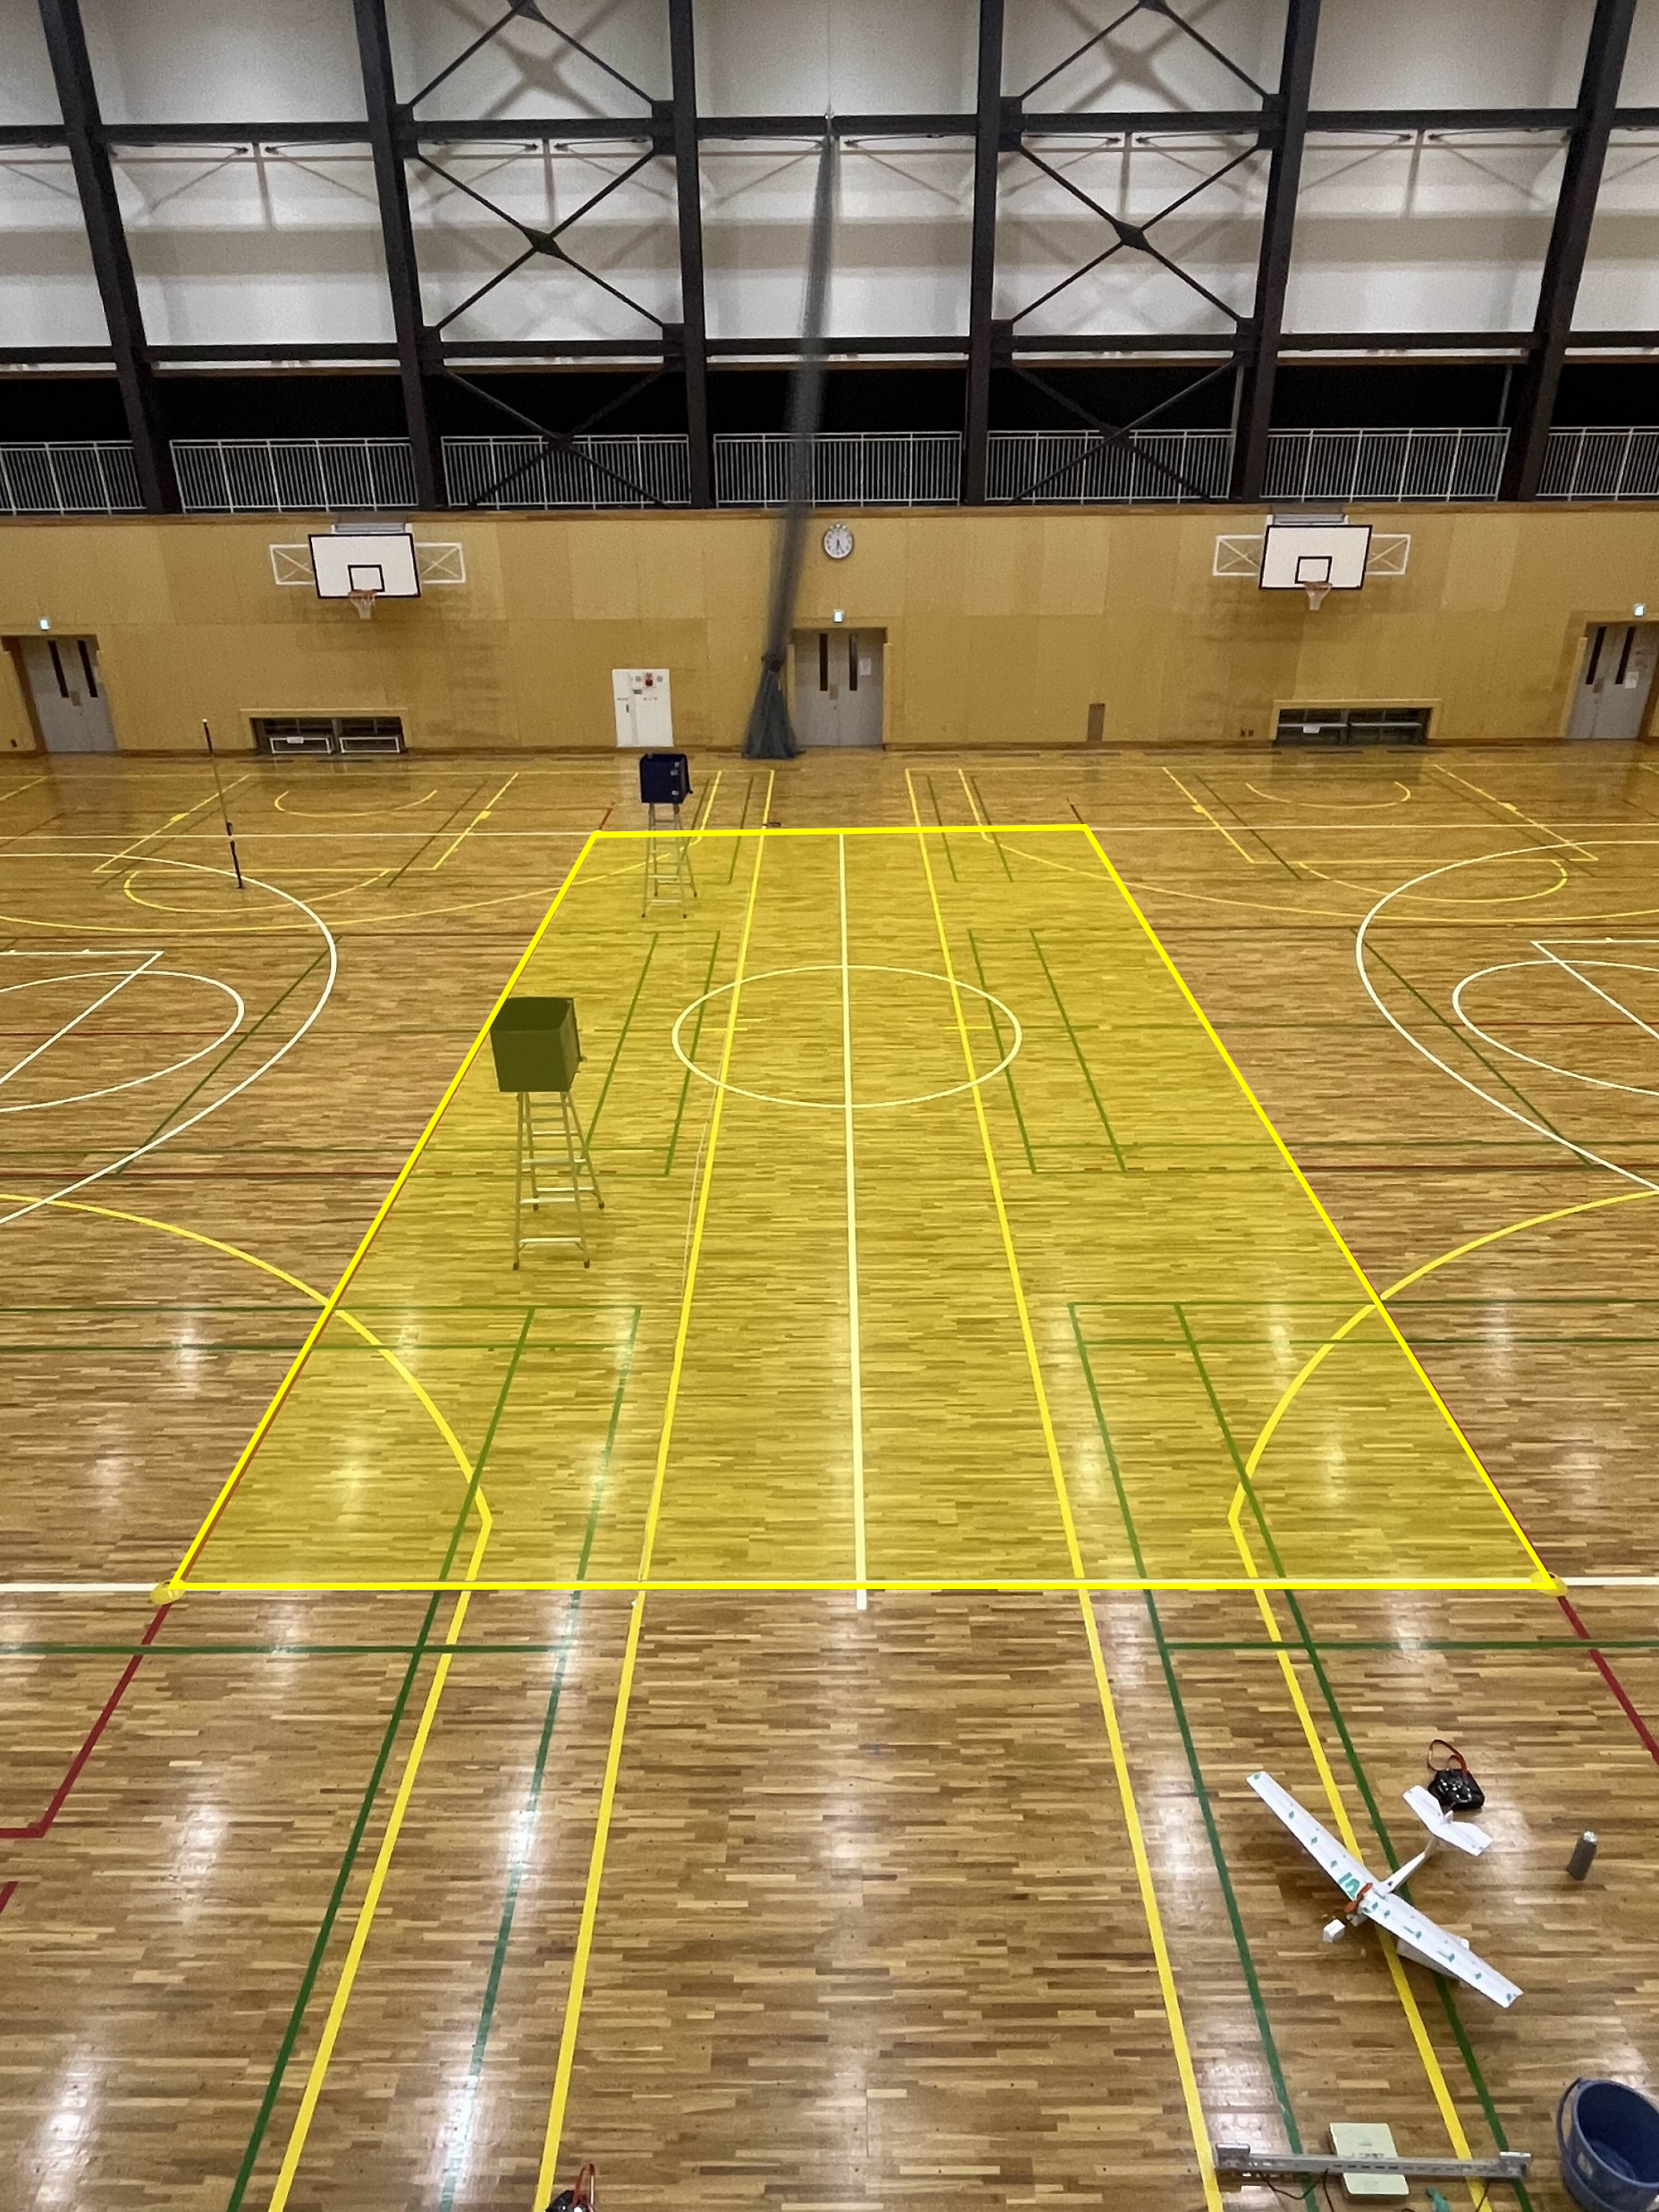
\includegraphics[width = 50mm,angle=90]{./multicopter_dropArea.png}
  \caption{物資投下エリア}
  \label{fig::multicopter::dropArea}
\end{figure}

\newpage
\subsubsection{8の字飛行用のポール}
8の字飛行で使用するポール周辺のフィールド図を図 \ref{fig::multicopter::poleTurn} に示す.
2本のポールの間(オレンジ線)をラインAとする.
ポールの外側(青線)をラインBとする.
\begin{figure}[h]
  \centering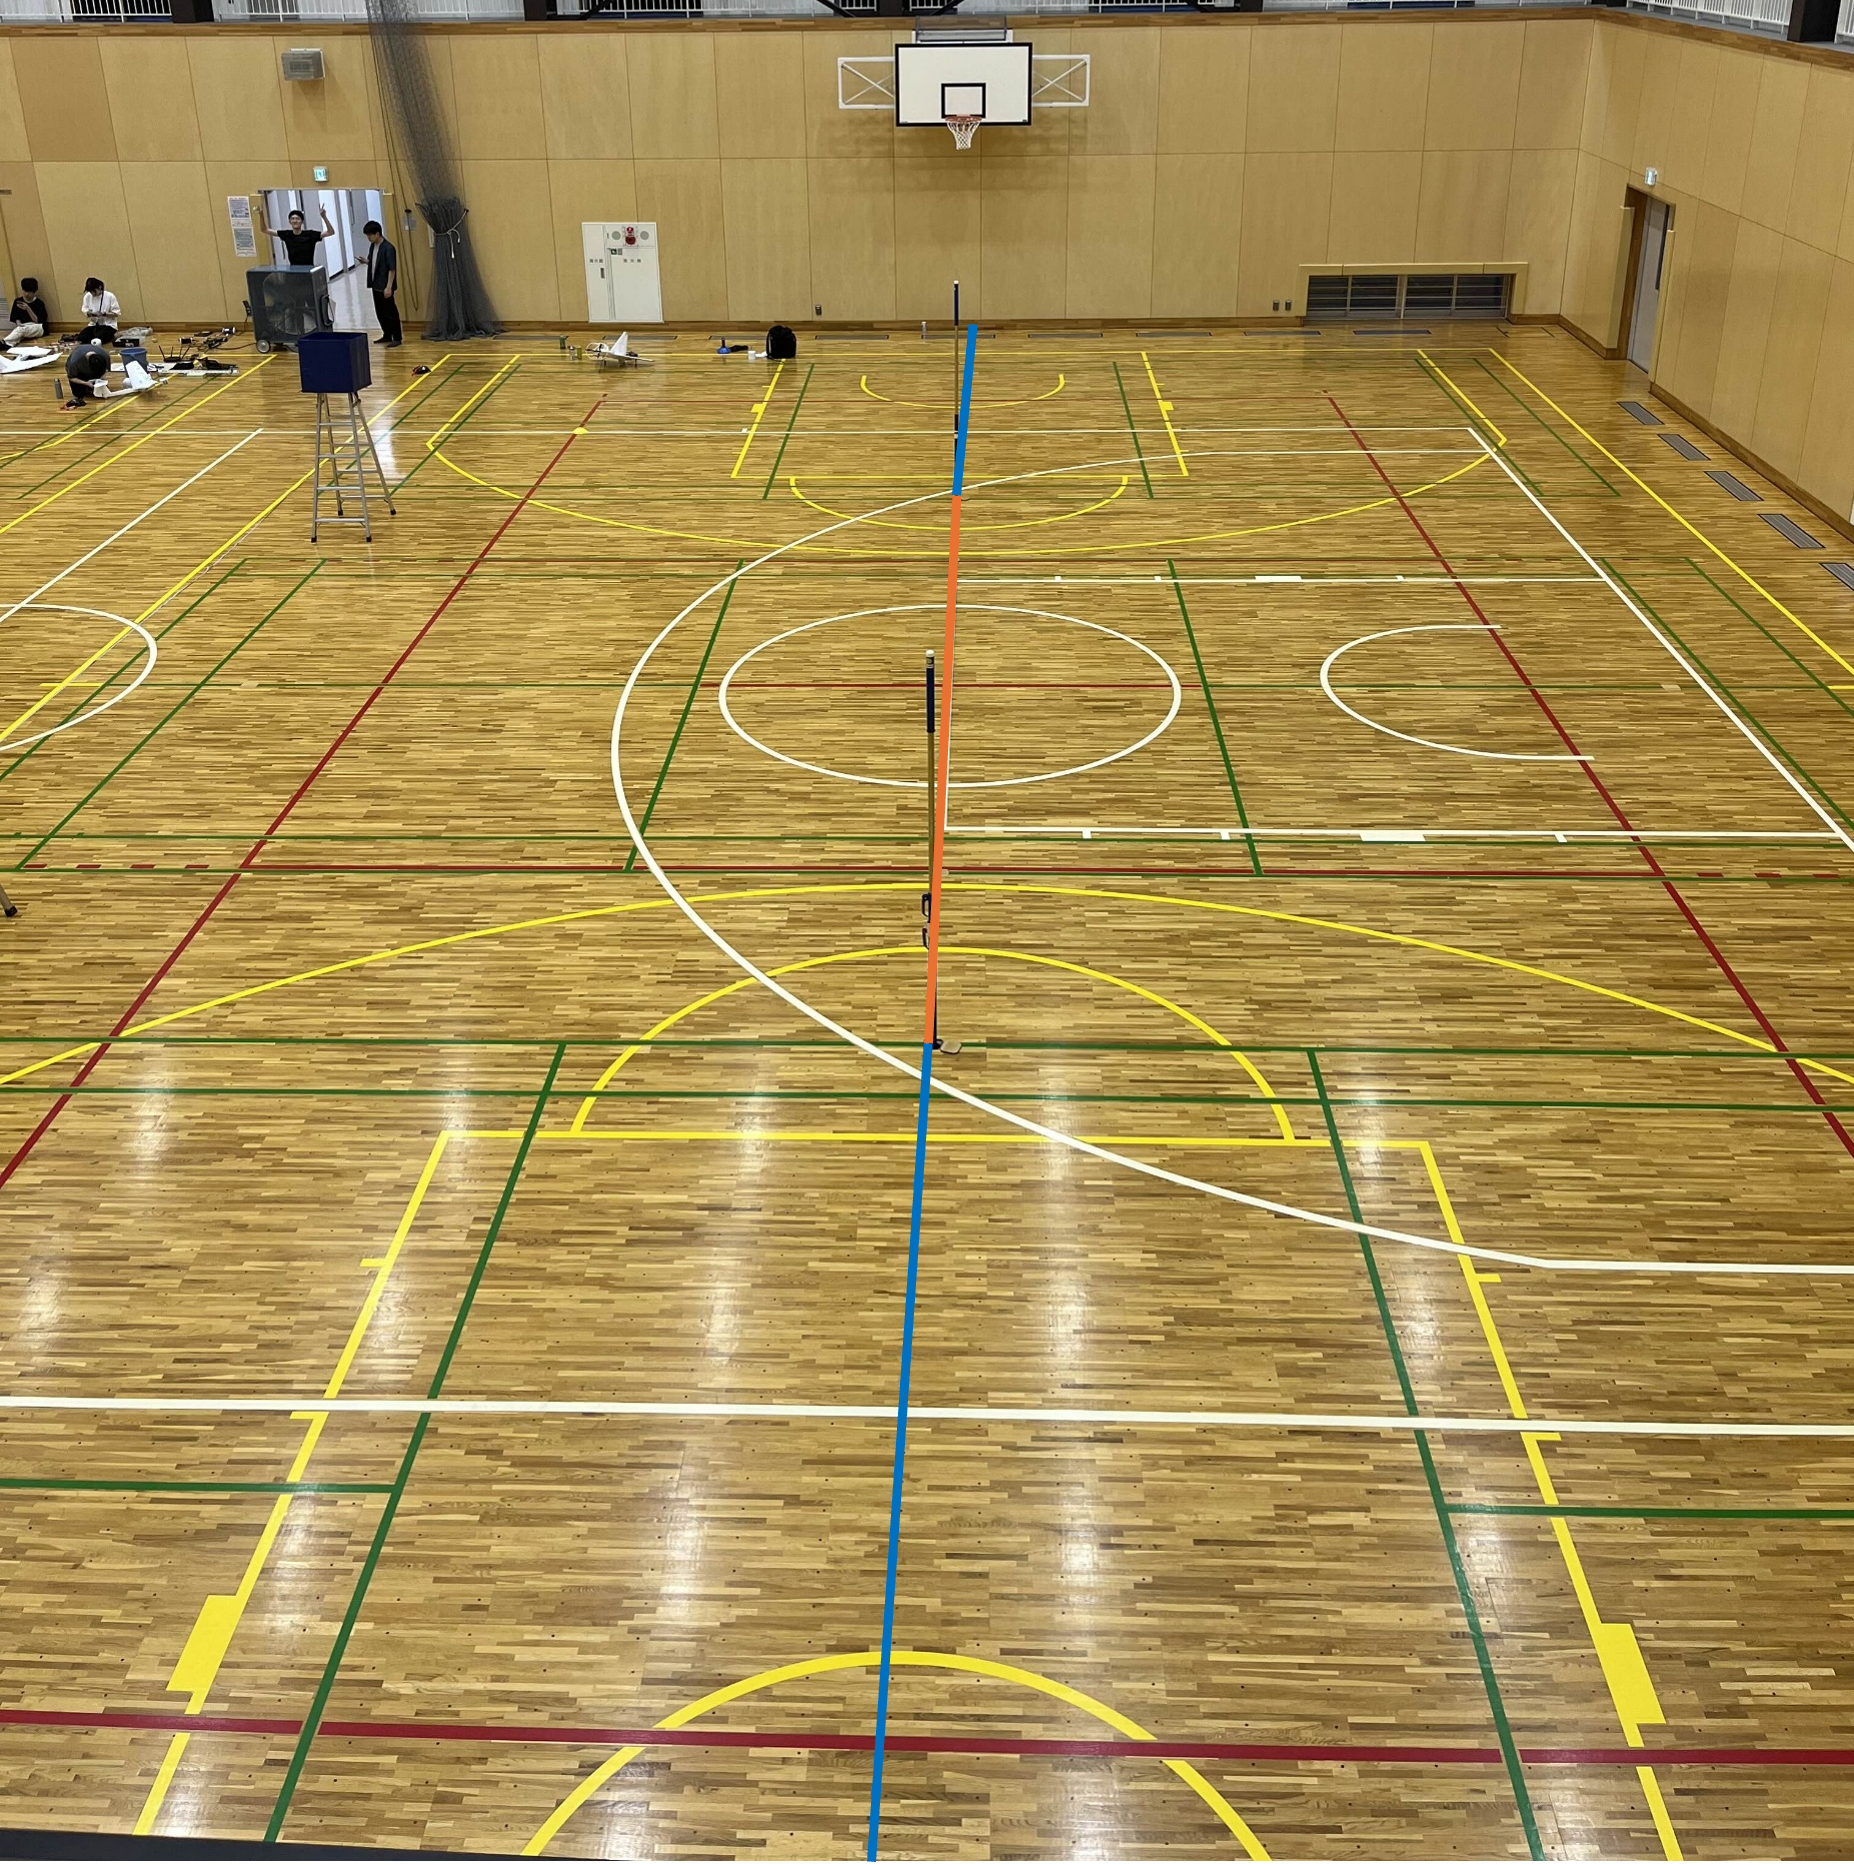
\includegraphics[width=70mm]{multicopter_poleTurn.png}
  \caption{8の字飛行用のポール}
  \label{fig::multicopter::poleTurn}
\end{figure}